\RequirePackage{xcolor}
\documentclass[a0]{sciposter} 
\usepackage{multicol}
\usepackage{graphicx,url,hyperref}
\hypersetup{hidelinks} 
\usepackage[spanish]{babel}   
\usepackage[utf8]{inputenc}
\usepackage{setspace}
\setlength{\parskip}{6pt}
\renewcommand{\arraystretch}{1.5}
\setstretch{1.1}

\title{Convocatoria de admisión}
\author{Doctorado en en Ingeniería de Sistemas}
\institute {Facultad de Ingeniería Mecánica y Eléctrica\\Universidad Autónoma de Nuevo León}
\email{admision-d@yalma.fime.uanl.mx}

\leftlogo[1]{uanl.png} 
\rightlogo[1]{fime.png}

\begin{document}

\conference{\raisebox{2cm}[0cm]{
\includegraphics[height=50mm]{pnpc.png}} \hfill \raisebox{2cm}[0cm]{
\includegraphics[height=50mm]{somosuni.png}}}

\maketitle

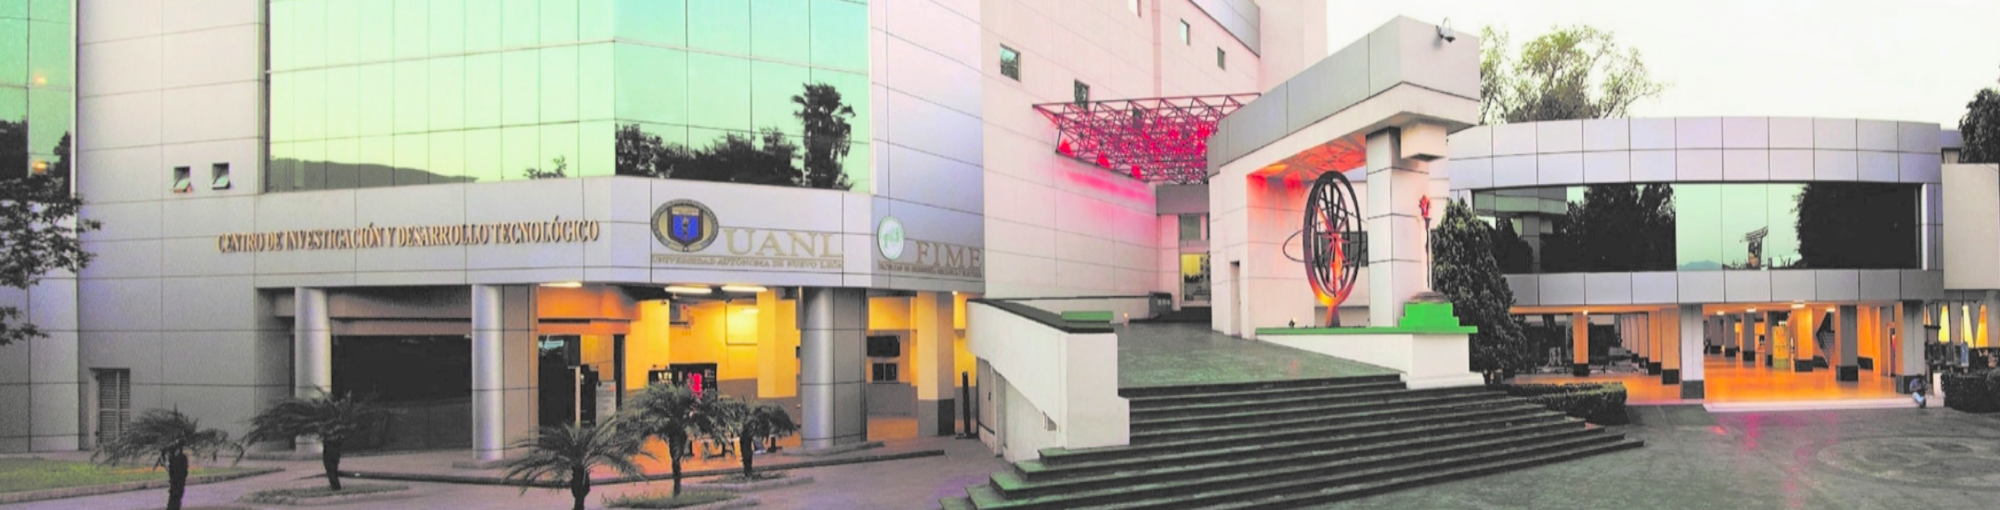
\includegraphics[width=\textwidth]{entrada.png}

\begin{multicols}{2} 

\section*{Propósito}

El Doctorado en Ingeniería de Sistemas es un programa de posgrado que
forma profesionistas altamente calificados capaces de llevar a cabo
investigación original de primer nivel y resolver efectivamente
problemas de sistemas de toma de decisiones que surgen en los sectores
productivos públicos y privados, mediante el modelado, análisis y uso
de técnicas cuantitativas.

\section*{Líneas de investigación}

\begin{itemize}
\item{Sistemas estocásticos y simulación}
\item{Métodos avanzados de optimización}
\item{Optimización de sistemas industriales}
\end{itemize}

Nuestra investigación aborda temas de optimización exacta y heurística
así como inteligencia computacional en aplicaciones de sistemas de
manufactura, logística, transporte, sistemas de producción, uso
eficiente de recursos naturales, servicios médicos y de salud,
biotecnología y agro-negocios, entre otras.

\section*{Requisitos técnicos de admisión}

\begin{enumerate}
\item{Poseer título de licenciatura en un área afín a la ingeniería,
computación o matemáticas.}
\item{Dominio del idioma inglés.}
\item{Entregar la siguiente documentación en formato PDF:
  \begin{itemize}
  \item{solicitud de admisión (disponible abajo)}
  \item{currículum vitae}
  \item{calificaciones del grado inmediato anterior}
  \item{anteproyecto doctoral avalado por un profesor investigador
    del programa}
  \item{cartas de recomendación por profesores o investigadores}
  \end{itemize}
  El formato de solicitud contiene mayor detalle sobre la
  entrega.}
\item{Entrevistarse con la Comisión de Admisión del programa.}
\item{Sustentar los tres exámenes técnicos del programa.}
\item{Sustentar los exámenes de admisión generales de la UANL:
  \begin{description}
  \item[EXANI-III]{Examen General de Conocimiento de CENEVAL}
  \item[EXCI]{Examen de Competencia en Inglés}
  \end{description}}
\end{enumerate}

\paragraph{Proceso de admisión}

La información para el registro como aspirante, para participar en el
proceso de admisión, requisitos administrativos y documentos/guías de
apoyo, alumnos extranjeros, pagos, se encuentra en
\url{https://www.uanl.mx/tramites/concurso-de-ingreso-a-posgrado/};
ahí mismo se debe realizar el registro para presentar los exámenes
EXCI y EXANI-III dentro de los Periodos de Admisión indicados en esta
Convocatoria.

Después de que la documentación del aspirante haya sido revisada, se
programará la entrevista por realizarse vía videoconferencia. La
admisión al Programa será determinada por la Comisión de Admisión y
estará basada en el expediente entregado; la rúbrica de evaluación
está enlazada abajo.

\section*{Fechas importantes}

\begin{tabular}{ll}
01/oct/21 &  Plazo para entrega de documentación \\
01-20/oct/21 & Registro para exámenes UANL: EXANI y EXCI$^*$ \\
25-28/oct/21 & Entrevistas y exámenes de PISIS \\
29-30/oct/21 & Exámenes UANL: EXANI-III y EXCI$^*$ \\
02/nov/21 & Publicación de resultados \\
17/ene/22 & Inicio de clases
\end{tabular}

$^*$ La información correspondiente al proceso de registro, pago,
fechas, guías de estudio y número de registro para el acceso a los
exámenes EXANI-III y EXCI se debe consultar en
\url{https://www.uanl.mx/tramites/concurso-de-ingreso-a-posgrado/} ya
que puede cambiar y no depende de PISIS.

\section*{Alumnos aceptados}

Los alumnos deben cubrir el pago de cuotas de inscripción a la UANL de
acuerdo con
\url{https://www.uanl.mx/tramites/costos-de-cuotas-escolares/} y
contar con Seguro Médico para el período enero-junio 2022.

\section*{Acreditaciones}

Este programa se encuentra acreditado por su calidad educativa y de
investigación por el Padrón Nacional de Posgrados de Calidad del
CONACYT.

\section*{Informes y correspondencia}

{\bf Comisión de Admision al Doctorado}\\
\href{mailto:admisión-d@yalma.fime.uanl.mx}{admisión-d@yalma.fime.uanl.mx}

\quad

{\bf Dr.\ César E. Villarreal Rodríguez} \\
{\em Coordinador Académico} \\
Tel.: +52 (81) 8329 4020 ext.\ 5945 \\
\href{mailto:cesar.villarrealrd@uanl.edu.mx}{cesar.villarrealrd@uanl.edu.mx }

\quad

{\bf Dr.\ Simón Martínez Martínez} \\
{\em Subdirector de Estudios de Posgrado} \\
\href{mailto:simon.martinez@uanl.edu.mx}{simon.martinez@uanl.edu.mx}

\end{multicols}

\quad

\begin{center}
\begin{tabular}{ccccc}
\quad & & \quad & & \quad \\
  

\includegraphics[width=80mm]{plan.png}
& &

\includegraphics[width=80mm]{solicitud.png}
& &

\includegraphics[width=80mm]{rubrica.png} \\

\quad & & \quad & & \quad \\
  
Plan de estudios & \quad\quad\quad &  Formato de solicitud & \quad\quad\quad & Rúbrica de evaluación \\
(descargar PDF) & & (descargar PDF) & & (consultar en línea) 


\end{tabular}
\end{center}



\end{document}
